\documentclass[times, twoside]{zHenriquesLab-StyleBioRxiv}
\usepackage{blindtext}
\usepackage[utf8]{inputenc}
\usepackage{graphicx}
\usepackage{mathtools}
\usepackage{blkarray, bigstrut}
\usepackage{bbold}
\usepackage{amsmath}
\DeclareMathOperator*{\argmax}{arg\,max}

% Please give the surname of the lead author for the running footer
\leadauthor{Denovellis} 

\begin{document}

\title{A state space model reveals the rich and varied dynamics of replay}
\shorttitle{Replay Dynamics}

% Use letters for affiliations, numbers to show equal authorship (if applicable) and to indicate the corresponding author
\author[1]{Eric L. Denovellis}
\author[2, 3]{Anna K. Gillespie}
\author[2, 3]{Michael E. Coulter}
\author[4]{Uri T. Eden}
\author[1, 2, 3, \Letter]{Loren M. Frank}


\affil[1]{Howard Hughes Medical Institute, University of California, San Francisco, San Francisco, California}
\affil[2]{Department of Physiology, University of California, San Francisco, San Francisco, California}
\affil[3]{Kavli Institute for Fundamental Neuroscience, University of California, San Francisco, San Francisco, California}
\affil[4]{Department of Mathematics and Statistics, Boston University, Boston, Massachusetts}

\maketitle

%TC:break Abstract
%the command above serves to have a word count for the abstract
\begin{abstract}
Representations of past or possible future experiences play a critical role in memory and decision-making processes. The hippocampus is a brain region known to express these representations across multiple states, including during sharp-wave ripple (SWR) events where sets of hippocampal place cells can be activated in time-compressed sequences consistent with a rapid mental traversal of a path. Efforts to understand these "replay" events typically analyze a small subset of events and assume rapid mental movement, and as a result we lack a clear picture of both the prevalence and the range of dynamics associated with replay. Here we develop a flexible state space model that uses a combination of discrete and latent states to capture the content and time evolution of SWR events. Application of this model reveals the large majority of SWR events contain coherent spatial content that evolves in accordance with a surprisingly wide range of mental movement speeds.

\end {abstract}
%TC:break main
%the command above serves to have a word count for the abstract

\begin{keywords}
Hippocampus | Replay | State Space
\end{keywords}

\begin{corrauthor}
%\texttt{loren{@}phy.ucsf.edu}
loren\at phy.ucsf.edu
\end{corrauthor}

\section*{Introduction}
The brain has the remarkable ability to retrieve representations of past events and generate representations of possible future events. These internal "generative" representations \cite{KayConstantSubsecondCycling2020} can be identified because the underlying neural activity patterns resemble those seen during actual events. In particular, an encoding model that relates neural firing to external covariates can be constructed during an experience, and this model can inverted to decode an internal representation of the covariates from the neural activity at a different time.

Mental events may not occur in the same time span as actual events; memories can be retrieved and used in less time than was required for the original experience, and mental simulations can span a series of actions more quickly than would be required to perform those actions. Consistent with this, generative representations can unfold rapidly. As a result, decoding generative representations often involves  making assumptions about their timescale and temporal structure, and these assumptions can limit the interpretation of the data. 

Hippocampal replay events are a prototypical example of a generative representation. As animals move through space, neurons in the hippocampus preferentially fire in at specific locations in an environment, and thus sets of cells can fire in sequence as the animal moves through a series of locations. When the animal is asleep or immobile, hippocampal cells can be reactivated during a "sharp-wave ripple" (SWR) event. A subset of SWRs contain sequential firing similar to that seen during a previous or potential future experience, and previous work has reported that these sequential firing events proceed at an average speed of ~10 meters / second, about 20x faster than the animal's usual movement speed \cite{DavidsonHippocampalReplayExtended2009}. 

Identifying these events typically involves multiple steps and assumptions about the nature of the event. First, an encoding model is constructed based on spiking activity during movement, most often using only spikes that have been clustered as single units (putative single neurons). Then, a subset of SWRs or events with high activity levels are selected based on an threshold for event size chosen by the experimenter. The spikes within these events decode the probability of position in overlapping or non-overlapping time bins whose size is also chosen by the experimenter. Finally, the most commonly used approach to detecting sequential replay involves fitting a line to the resulting set of probability distributions, which instantiates the assumption that the representations progress at a constant speed. A statistical test is then used to determining whether the fit is better than the fit to shuffled versions of the data.

While this approach identifies constant speed events, it does not consider events that are rejected by the statistical test, and the use of a fixed size temporal bin acts as a boxcar smoother that limits the potential movement speeds of the representation. The linear fit is also problematic, because it has the potential to reject real events that do not move at constant speeds. Moreover, there is now evidence that a subset of these events have stationary representations of a single location, which are often excluded. In addition, these methods identify only a subset of events as containing content (typically somewhere between 10 and 45\% of the chosen events), and thereby provide little insight into the remaining majority of the events.

 Recognizing the problems with the linear fit, several studies have moved away from the constant velocity assumption, using the weighted mean or maximum of each posterior time bin and connecting each time bin with a line. For example, using this approach, Pfeiffer and Foster \cite{PfeifferAutoassociativedynamicsgeneration2015} found that replays can alternate between representing a single location and sequential spatial trajectories. On the other hand, Stella et al. \cite{StellaHippocampalReactivationRandom2019} found that replays are more spatially continuous, following Brownian diffusion dynamics. Both methods still used large time bins and neither took into account the uncertainty of the decoded estimates, making it hard to identify the source of the different conclusions.

An ideal approach to identifying and quantifying the dynamics of generative representations would circumvent these problems. It would use all of the available spiking data to yield the most accurate decoded positions. It would be applicable to either thresholded events or to all of the data to permit an unbiased assessment of the prevalence and nature of generative activity. It would use very small temporal bins (1 or 2 ms) to allow for very rapid representational movement and provide information about the certainty of the decoded estimates. It would be able to capture different types of movement dynamics, ranging from stationary to rapidly evolving to disorganized, and provide a statistical assessment of confidence for the dynamic. Finally, where assumptions are made, it would provide well defined parameters whose values can be explored systematically to understand their influence on the results.

We therefore developed a state space model of generative activity that achieves all of those goals. State space models are a well-understood, well-known statistical solution to the problems described above. By mathematically modeling the relationship between the data and latent dynamics, state space models make the assumptions of the model explicit and interpretable. Our model goes beyond previous approaches \cite{MaboudiUncoveringtemporalstructure2018, DengRapidclassificationhippocampal2016} and characterizes represented trajectories as a mixture of three underlying patterns of dynamics: stationary trajectories, continuous trajectories that are many times the typical speed of the animal, and spatially fragmented trajectories. We show how this model can take advantage of clusterless decoding---which relates multiunit spike wave form features to position without spike sorting---giving us more information about the population spiking activity. We apply this model to data from 10 animals, focusing on SWR events to permit a direct comparison to previous work. We find that the vast majority of SWRs contain spatially coherent content. Surprisingly, while the expected high speed replay events were identified, the most common category of events expressed representations that moved at speeds consistent with real animal movement, suggesting that high speed replay is not the most common manifestation of generative activity. Our method provides a useful and powerful tool for understanding the dynamics of mental representations, and could be adapted for use in many brain areas. 

\section*{Results}
\begin{figure*}%[tbhp]
\centering
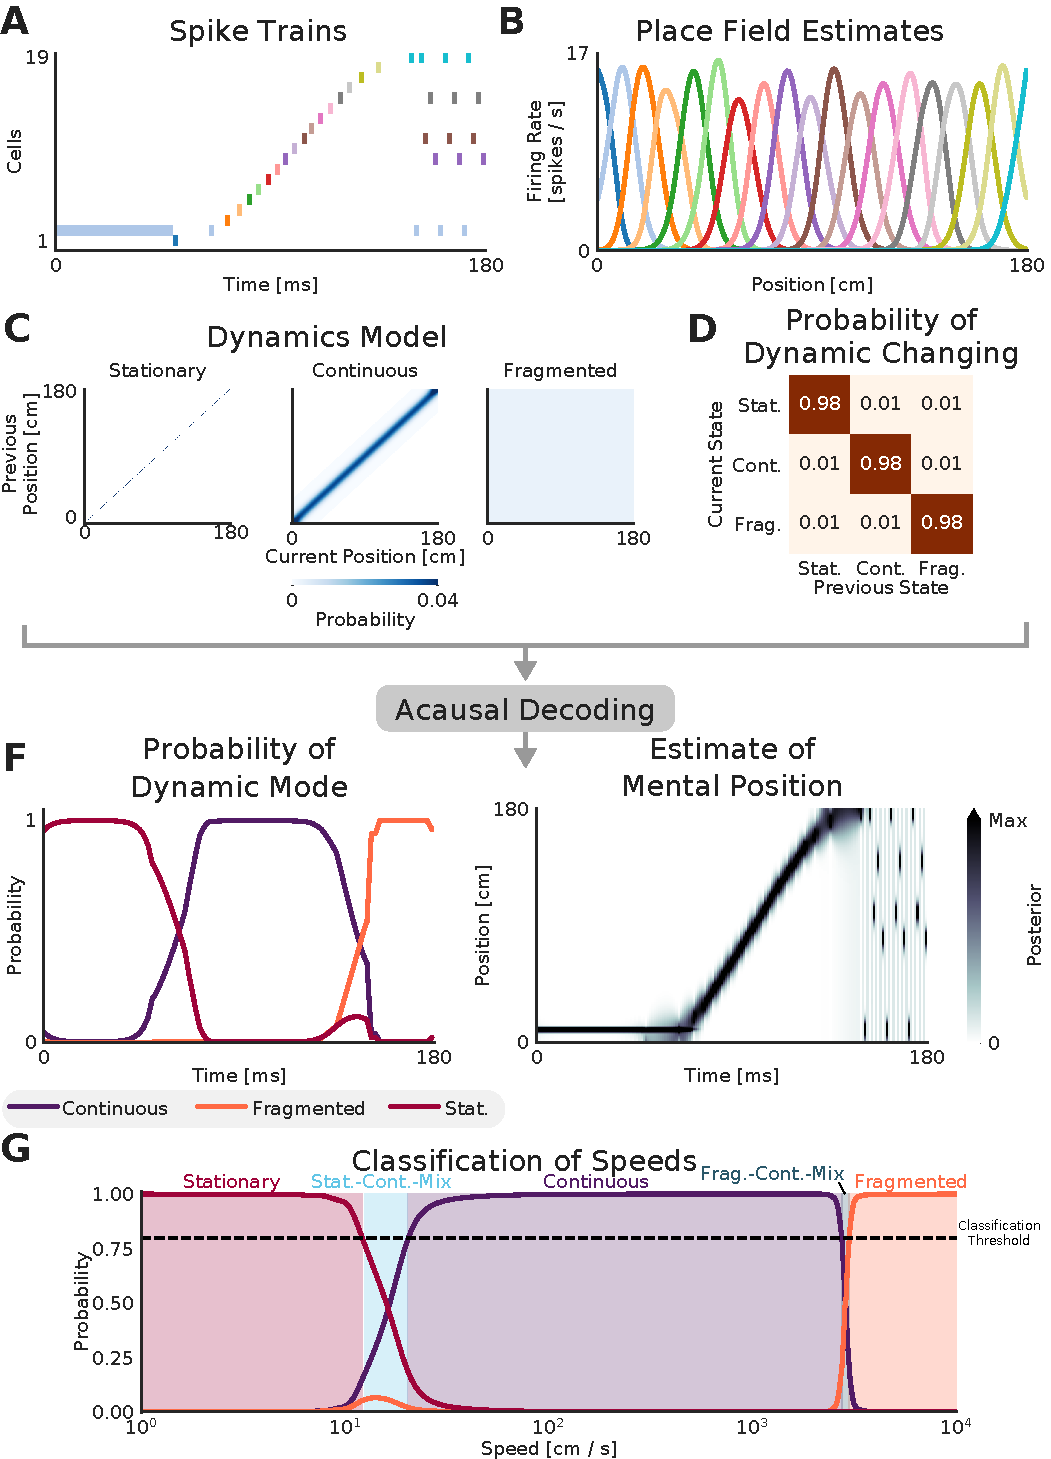
\includegraphics[width=0.80\linewidth]{figures/Figure1/Figure1_v4}
\caption{Components of the state space model and demonstration on simulated data. \textbf{(A)} 19 simulated place cells that exhibit three different sequence patterns. For the first third of time, one cell fires repeatedly, representing one stationary location. For the second third of time, the cells fire in sequence, representing a smooth continuous trajectory through space. For the last third cells fire in an incoherent pattern, representing a non-smooth fragmented trajectory through space. \textbf{(B)} Like the Bayesian Decoder, the state space model uses estimates of cells' place fields from when the animal is moving and combines them with the observed spikes in (A) to compute the likelihood of position for each time step. \textbf{(C)} This is combined with an explicit model of each dynamic state--which determines how latent position can change based on the posterior from the previous time step. In the stationary state, this is modeled as the identity matrix because the position remains the same. In the continuous state, the dynamics are modeled as a Gaussian random walk, meaning the next possible position is likely to be spatially close. In the fragmented state, the dynamics are modeled as uniform, meaning the next position is equally likely to be anywhere. Note that the dynamics displayed only reflect the within-state dynamics. \textbf{(D)} The probability of remaining in a particular state versus switching to another state. This is modeled as having a high probability of remaining in a particular state with a small probability of switching to one of the other dynamics at each time step. \textbf{(F)} The state space model uses the components in A-D over all time to decode the joint probability of latent position and dynamic state. The joint probability can be summarized by marginalizing over latent position (left panel) to get the probability of each dynamic state over time (lines). This can also be used to get an estimate of latent position over time (right panel). \textbf{(G)} The probability of each state given a particular constant speed trajectory. Each speed corresponds to a simulated spiking sequence at that speed. The lines correspond to the average probability of that state over the sequence. Dotted line represents the 0.8 classification threshold we use to classify each range of speeds and shaded regions correspond to the classification we have given the range of speeds.
}
\label{1}
\end{figure*}
\subsection*{Overview of the model}
We begin with an application of the model to simulated data, both to validate the model and to provide intuition. (Figure \ref{1}). We simulated 19 Poisson spiking cells with Gaussian place fields on a 180 cm virtual linear track. Each place field has a 36 cm variance and a 15 Hz peak firing rate, which is spaced every 10 cm along the virtual track. We then apply our decoding algorithm to the spiking sequence in Figure \ref{1}A. For the first third of this sequence, a single place cell fires repeatedly, representing a single location. For the middle third of the sequence, the cells fire in sequential spatial order, representing a fast moving trajectory. For the last third, the cells fire in a incoherent spatial order. These firing patterns represent three different types of sequence dynamics that could be expressed during replay events, which we call stationary, continuous, and fragmented, respectively. The goal of our model is to characterize SWRs in terms of a mixture of these three dynamics at every time point.

Decoding the spiking sequence dynamics requires specifying two elements: the data model---how the spikes relate to position---and the dynamics model--how the position can change over time. For the data model, our decoder is the same as the Bayesian decoder. We compute an estimate of how each cell's firing rate varies over position (the place field, Figure \ref{1}B). This is used during decoding to compute the Poisson likelihood of position over time given the spiking sequence of interest. In contrast to the Bayesian decoder, we can use arbitrarily small time bins (in our case 2 ms vs. 20 ms or more) because we are able to take advantage of the prior placed on the dynamics by the state space model. This allows us to detect changes on smaller time scales than would be possible with the Bayesian decoder.

Next, we specify a dynamics model for how latent position---the "mental" position of the animal represented by the cells--- evolves over time (Figure \ref{1}C). We do this by defining a movement state transition matrix, which defines how the latent position can change from the previous time step. Previous findings suggest three distinct dynamics: stationary \cite{JaiDistincthippocampalcorticalmemory2017, FarooqEmergencepreconfiguredplastic2019}, smoothly moving \cite{DavidsonHippocampalReplayExtended2009}, and fragmented / jumpy \cite{PfeifferAutoassociativedynamicsgeneration2015}, which could correspond to both spatially incoherent representations and representations that jump from one position to another. We therefore developed state transition models to capture each of these dynamics.

In the stationary dynamic, the latent position would not change between time steps, so we use an identity state transition matrix, which predicts the next position will be the same as the last position. In the continuous dynamic, the latent position would be "spatially close" to the position in the previous time step, so we use a Gaussian random walk state transition matrix. This means that, for a given latent position, the probability of moving to another position is modeled by a Gaussian centered at that position and "spatially close" is defined by the variance of the Gaussian. In our case, since we are interested in identifying replays that move at speeds much faster than the animal's speed, we set this to 6.0 cm. This ensures that with a 2 ms time step, the latent position is 95\% likely to be within 4.90 cm of the previous latent position (corresponding to a latent speed of up to ~25 m/s). This is consistent with replay speeds observed in previous studies \cite{DavidsonHippocampalReplayExtended2009, PfeifferAutoassociativedynamicsgeneration2015}. Finally, in the fragmented dynamic, the latent position could move to any available position instantaneously. We model this using a uniform state transition matrix, which makes all positions equally likely.

Finally, we specify how likely the dynamic is to persist in time versus changing to another dynamic (Figure \ref{1}D). In order to be conservative, we assume that each dynamic is likely to dominate for the duration of the SWR, with a small probability of switching to one of the other dynamics (note that below we show that our results are relatively insensitive to this parameter). Accordingly, we set the probability of staying in a state to 0.98 for each 2 ms time step. Because the probability of changing dynamics follows a geometric distribution, this corresponds to an expected duration of 100 ms for staying in a particular state.

Once we have specified the data and dynamics model, we have fully specified the state space model. We use acausal decoding, meaning that we use all information from the past and future spikes, to estimate the joint posterior probability of position and dynamic state (see Methods). With this, we can summarize the resulting posterior with two quantities: the mixture probability of each dynamic over time and the probability of position over time, irrespective of dynamic (Figure \ref{1}F, left and right plot respectively). 

An examination of these two summaries reveals that that the model successfully captures the dynamics of the population spiking activity in Figure \ref{1}A. The stable firing of the one active neuron indicates a stationary representation, and the probability of the stationary dynamic is high at the beginning of the simulated replay. The change in the data then drives a rapid transition to the continuous dynamic, reflecting the trajectory-like spiking from the population of cells. Subsequently, as the population activity becomes spatially incoherent, the fragmented dynamic dominates for the last third. Importantly, these dynamics also inform the estimate of latent position of the animal, and the correct assignment of dynamic reduces the variance of the latent position estimate.

The specification of these dynamics allows the model to capture a wide range of movement speeds for the latent position. To demonstrate this, we applied the model to simulated trajectories of increasing speed (Figure \ref{1}G), from 1 cm/s to 10,000 m/s. From this, we can see that not only are there regions of speed that correspond to our three dynamics being high probable (where we define highly probable to be over 0.8 probability), there are intermediate speeds where two of the dynamics dominate with high probability; that is, the sum of two of the dynamics' probabilities is over 0.8. In this manuscript, we will refer to these as mixture dynamics. For example, when the stationary state has a probability of 0.6 and the continuous has a probability of 0.4, we call this a stationary-continuous mixture (light blue, Figure \ref{1}G). By using this classification scheme, we can characterize the speed or set of speeds in a replay by its dynamics.

We note here that the choice of any particular threshold is arbitrary, and that the power of our approach lies in part in the ability to assign a confidence value for each dynamic or combinations of dynamics to each moment in time. Our goal in choosing 0.8 was to use a threshold that corresponds to highly probable and to explicitly avoid the arbitrary choice of 0.95 because the 0.95 threshold often leads people to conclude that only events that are statistically significant at the 0.05 level are likely to be meaningful to the brain. Nonetheless, we also verified that our central results hold with a higher threshold of 0.95. 

As mentioned above, the model is robust to the choice of probability of staying in a state. We decoded the spiking sequence in Figure \ref{1}A with different probabilities of staying in the same state versus switching to another state (Figure 1-Supplemental Figure 1). We found that for a large range of plausible probabilities of staying in one of the dynamics (0.9 - 0.9999), the model still correctly identified the dynamic with high probability.

\begin{figure*}%[tbhp]
\centering
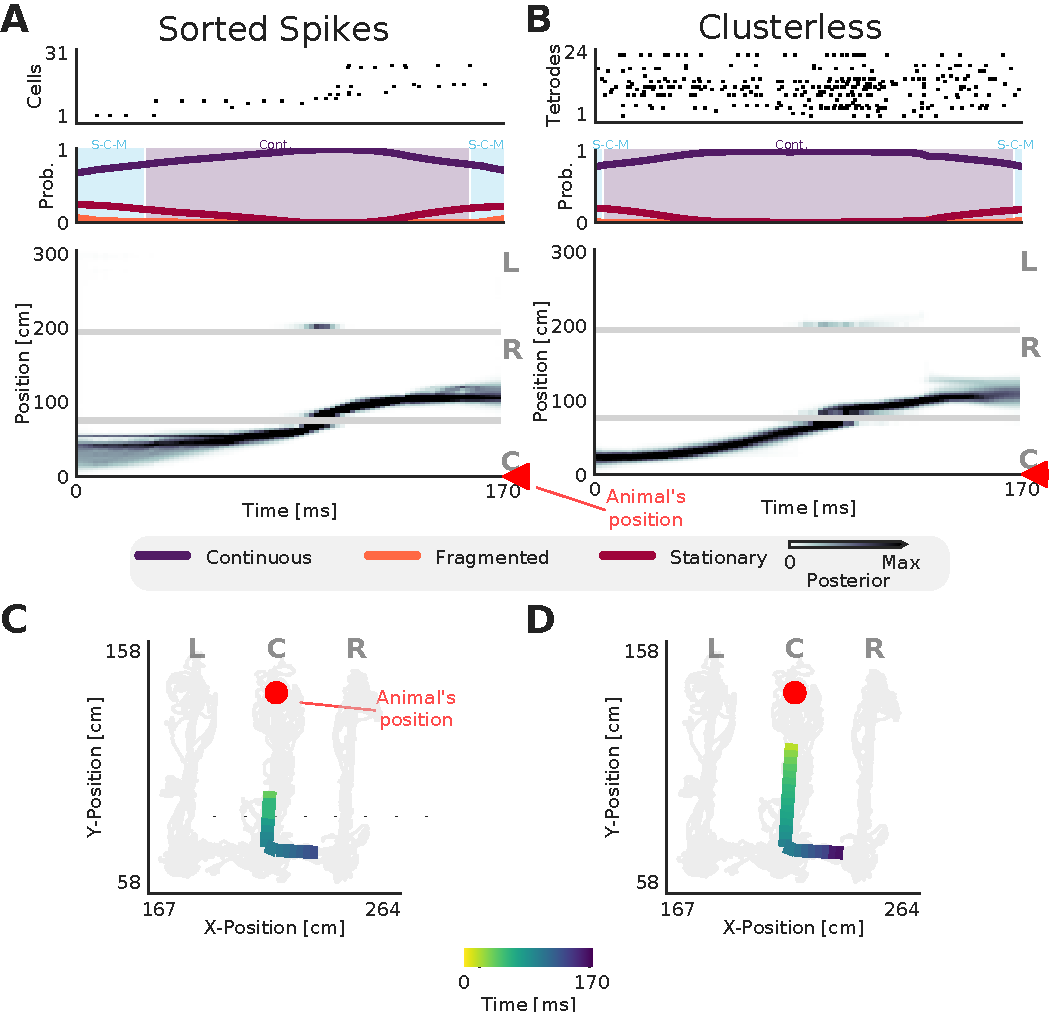
\includegraphics[width=0.80\linewidth]{figures/Figure2/Figure2_v4}
\caption{Demonstration of the state space model on real data using both sorted and clusterless spikes on the same SWR. \textbf{(A)} Decoding using sorted spikes. The top panel shows 31 cells on a W-track ordered according to linearized position by their place field peaks. The second panel shows the probability of each dynamic over time as in Figure 1F. Shaded regions correspond to the speed classifications as in Figure 1G. The third panel shows the estimated probability of latent position over the course of the SWR as it travels down the center arm toward the right arm. L, R, C correspond to the position of the left, right and center reward wells respectively. The animal's actual position is indicated by the red triangle. \textbf{(B)} Decoding using clusterless spikes. The top panel shows multiunit spiking activity from each tetrode. Other panels have the same convention as(A).  \textbf{(C)} 1D MAP estimate of the latent position in (A) projected back into 2D. Color indicates time. The animal's actual position is denoted by the red circle. Light grey lines show the animal's 2D position over the entire epoch. L, R, and C correspond to the left, right and center reward well as in (A). \textbf{(D)} 1D MAP estimate of the latent position in (B) projected back into 2D. Figure conventions are the same as in (C).
}
\label{2}
\end{figure*}
\subsection*{Identification of continuous replays with sorted and clusterless spikes}

\begin{figure*}%[tbhp]
\centering
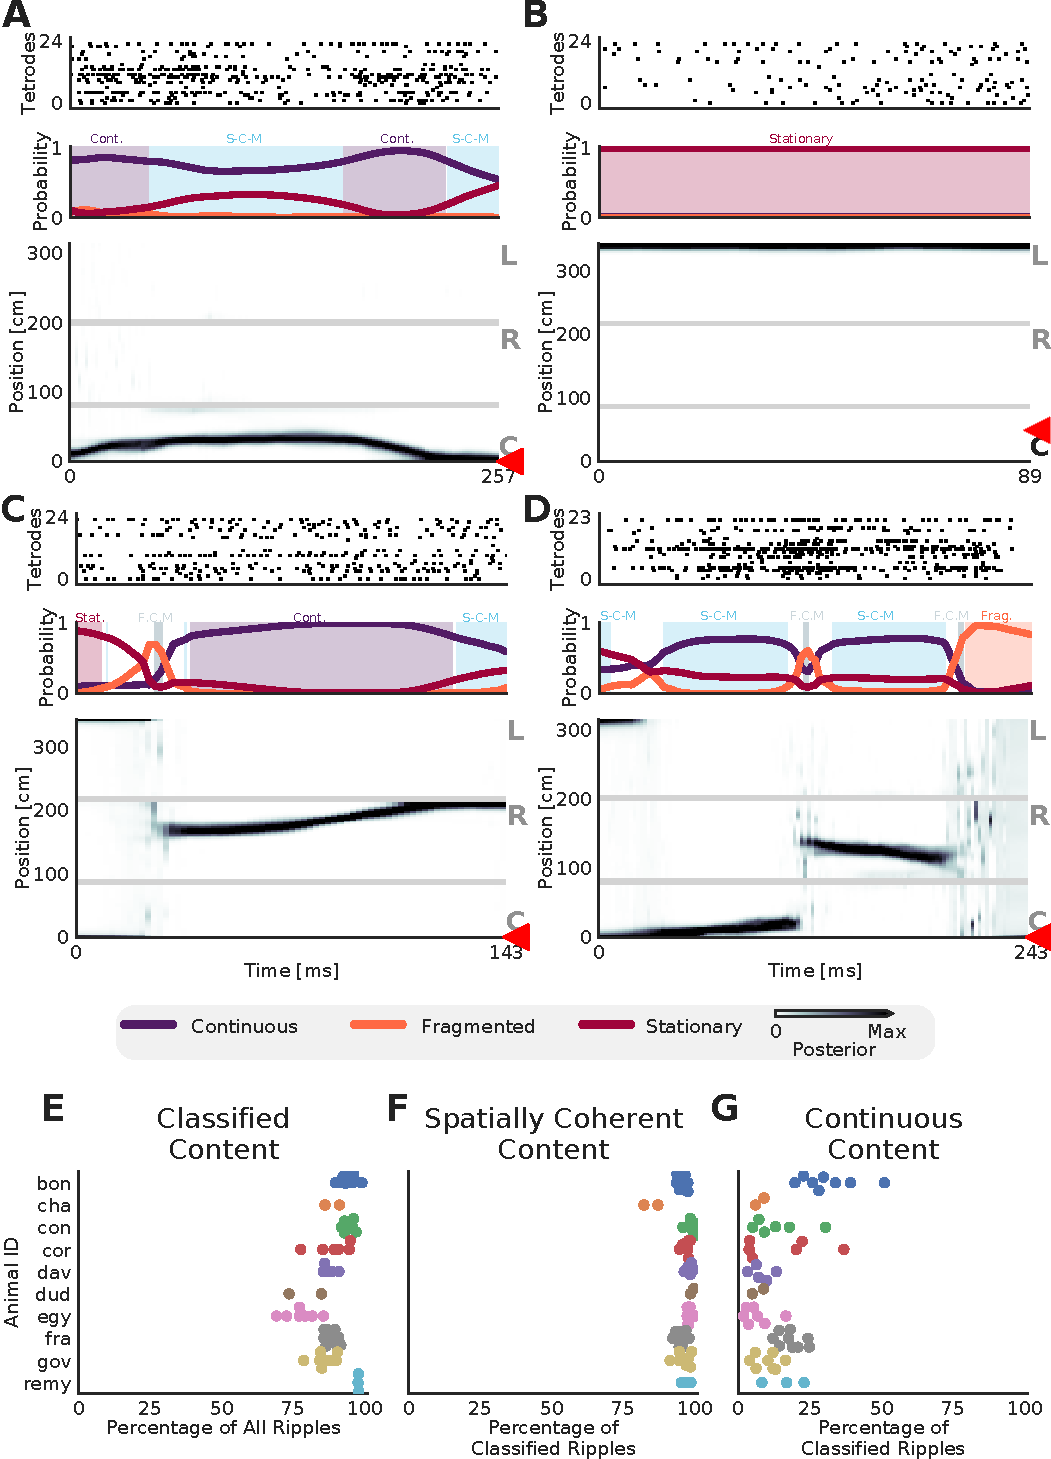
\includegraphics[width=0.80\linewidth]{figures/Figure3/Figure3_v4}
\caption{A-D. Four examples of replays that would not be well-characterized by using the Bayesian decoder. Figure conventions are the same as in Figure 2. \textbf{(A)} A replay that starts down the center arm away from the animal's position at the center well, slows down, and returns back. \textbf{(B)} A replay that stays at the left well for the entirety of the SWR while the animal is in the center arm. \textbf{(C)} A replay that begins stationary at the left well and then jumps to the middle of the right arm and proceeds up the right arm to the right well. \textbf{(D)} A replay that begins stationary at the left well, jumps to the center arm, proceeds away from the center well, jumps to the right arm, proceeds back toward the center well, and then becomes fragmented. \textbf{(E)} Percentage of SWRs in each epoch that has some content that falls into one of the categories (Stationary, Stationary-Continuous-Mix, Continuous, Fragmented-Continuous-Mix, or Fragmented). \textbf{(F)} Of the classified content, the percentage of SWRs in each epoch that have some Stationary, Stationary-Continuous-Mix, or Continuous content. \textbf{(G)} Of the classified content, the percentage of SWR in each epoch that has some Continuous content.
}
\label{3}
\end{figure*}

Our success with simulated data inspired a further validation of the model on real hippocampal data. We fit the place fields of 31 cells recorded in hippocampus while the rat was performing a spatial alternation task on a W-shaped track, and then applied the decoding algorithm to a SWR with sequential population activity (Figure \ref{2}A, top panel). As expected, we observed that the probability of being in the continuous dynamic is high throughout this SWR, but the probability of being in a stationary state was noticeable at the beginning and end of the SWR (Figure \ref{2}A, middle panel). Using our speed classification scheme, this means that the speed of the replay starts slower---as a mixture of continuous and stationary dynamics---and then speeds up and slows down again. This is also evident in the posterior probability of linear position over time. This shows that the replay travels down the center arm and up the right arm (Figure \ref{2}A, bottom panel). We can also see this when we project the maximum of the posterior of this trajectory to 2D (Figure \ref{2}C) to better see the spatial trajectory. Moreover, when we apply the same model using the 2D position of the animal, we get a similar result as when we used the 1D linearized position (Figure 2-Supplemental 1A).

One of our criteria for a more optimal method is that it use all of the available spiking data. Using only clustered spikes discards all of the spike events that cannot be uniquely assigned to a putative single neuron, substantially reducing the quality of the resulting decoding. Additionally, spike sorting is not necessary to recover the underlying neural population dynamics \cite{TrautmannAccurateEstimationNeural2019}. We therefore adopted a "clusterless" approach which directly relates spikes and their multiunit spike waveform features to position without spike sorting, which we call clusterless decoding (see Methods). Clusterless decoding previously has been used to successfully identify theta sequences and replay sequences in the hippocampus (\cite{KloostermanBayesiandecodingusing2014, ChenTransductiveneuraldecoding2012,DengRapidclassificationhippocampal2016, KayConstantSubsecondCycling2020}). Applying a clusterless decoder to the same SWR, we get similar classification of the sequence (Figure \ref{2}B, D), both with 1D linearized position and 2D position (Figure 2-Supplemental 1B). The spatial extent of the event is longer and the estimate of the posterior probability of position is narrower for the clusterless model, however. This reflects the clusterless model's access to a larger pool of data that provides more information about the extent of the event, and more certainty in the latent position and the dynamic (Figure \ref{2}D vs C).

\subsection*{Replays with non-constant speed}

After testing our model on a single SWR, we applied our decoding algorithm to hippocampal recordings from 10 animals performing the W-track spatial alternation task (tetrodes = [10, 24], brain areas = [CA1, CA2, CA3]; some data previously used in \cite{KarlssonAwakereplayremote2009, KayConstantSubsecondCycling2020}). One major goal of our work was to assess the overall prevalence of spatial content across SWRs, so we detected SWRs using a relatively permissive threshold (see Methods) to ensure that we were included both the rare large events as well as the much more common small events. 

As expected, and providing further support for the validity of the method, we observed many replays that were classified as continuous throughout the entirety of SWR (Figure 2-Supplemental 2A-C). However, we also observed many events with spatially coherent content that did not have this structure. For example, there were trajectories that started in one direction and reversed back to the original position (Figure \ref{3}A, Figure 3-Supplemental 1B), trajectories that remained fixed in one position (Figure \ref{3}B), trajectories that jumped between arms and between dynamics (Figure \ref{3}C-D, Figure3-Supplemental 1A, E, F), and trajectories that were spatially incoherent throughout the SWR (Figure3-Supplemental1D).

Using our 0.8 threshold, we were able to classify 89\% ( 23382 of 26160) of SWRs as containing at least one of the five dynamics. To ensure that this depended on the spatial receptive fields of cells in the hippocampus, we resampled position with replacement for two epochs, shuffling the relationship between spiking and spatial information. We then decoded the same SWR events containing the same spikes. Only 9\% of the SWRs were classified in the shuffled datasets, a value that was significantly less than that seen for the real data (p=0.02 for epoch 1, p=0.02 for epoch 2, Figure 3-Supplemental 2).

Previous work focusing on spatially sequential replay reported that only a minority of events contain sequential spatial content [REFS]. We therefore asked what fraction of classified events contained spatially coherent content in any form, defined as a SWR containing any times with stationary, stationary-continuous mixture, or continuous dynamics (see Methods). We found that 22478 of 23382 or 96\% of classified SWRs had time points with spatially coherent structure. We then asked what fraction of events contained spatially incoherent content, defined as a SWR containing any times with fragmented-continuous mixture or fragmented. We found that only 3353 of 23382 or 14\% of classified SWRs had time points with spatially incoherent structure. This was consistent across animals (Figure \ref{3}F). We then asked what percentage of classified SWR contained continuous content, like would typically be analyzed when using the Bayesian decoder. Here our findings were consistent with previous reports: in our datasets 4511 of  23382 or 19\% of classified SWRs had some continuous content (Figure \ref{3}G). Thus, focusing on only continuous content misses a large fraction of events where there is evidence for spatially coherent, but not continuous content.

We repeated this analysis with a higher threshold of 0.95 to ensure that our result was not dependent on this threshold. We found that, while this slightly reduced the total fraction of classified ripples (19180 / 25845 or 74\% SWRs), an even higher fraction of the classified ripples (19020 / 19180 or 99\% classified) had spatially continuous content. Classified SWRs containing spatially incoherent content similarly were a small fraction of the classified SWRs (spatially incoherent: 484 / 19180 or 3\%).

Our model is specified in the context of a latent position associated with different dynamics. This specification allows us to not only decode events, but also to quantify the model's certainty in each position estimate at each moment in time given the model parameters. To do so we can compute the cumulative spatial extent of the 95\% highest posterior density (HPD) values of the posterior linear position. Larger values of the cumulative HPD indicate the model is less certain about position, because the HPD values are spread out over more of the track at a given time point, whereas lower values indicate that the model is more certain about the estimate of position, because the HPD values are more concentrated and cover less of the track. Thus, the HPD provides a complementary measures of spatial coherence, and evaluating it allows us to verify that the events we defined as spatially coherent correspond to events where there is high certainty around the position estimates.

We found that spatially coherent events did indeed have lower cumulative HPDs. Figure \ref{4}A and B show two example SWRs that were classified as having stationary and continuous dynamics, respectively. The bulk of the HPD values at each time step in these SWRs is concentrated in a small portion of the track and the cumulative HPD is low throughout the SWRs. In contrast, Figure \ref{4}C shows a SWR where the dynamics are fragmented and correspondingly, the HPD is much more spatially diffuse and the cumulative HPD is much higher. The HPD also provides insights into the moment-by-moment structure of each event, which can change over the time course of a SWR. An example of this change is shown in Figure \ref{4}D, where the cumulative HPD is small for most of the SWR until the end, where the uncertainty of position becomes much higher, reflecting a transition from a spatially coherent to a spatially incoherent representation. Overall, when we examined the average cumulative HPD for each SWR, grouped by dynamic, we found a clear bi-modal split between spatially coherent dynamics and spatially incoherent dynamics (Figure \ref{4}E). For the spatially coherent dynamics, the cumulative HPD was much lower than the spatially incoherent dynamics (median 24 cm, spatially coherent vs. median 238 cm, spatially incoherent).

\begin{figure*}%[tb2]
\centering
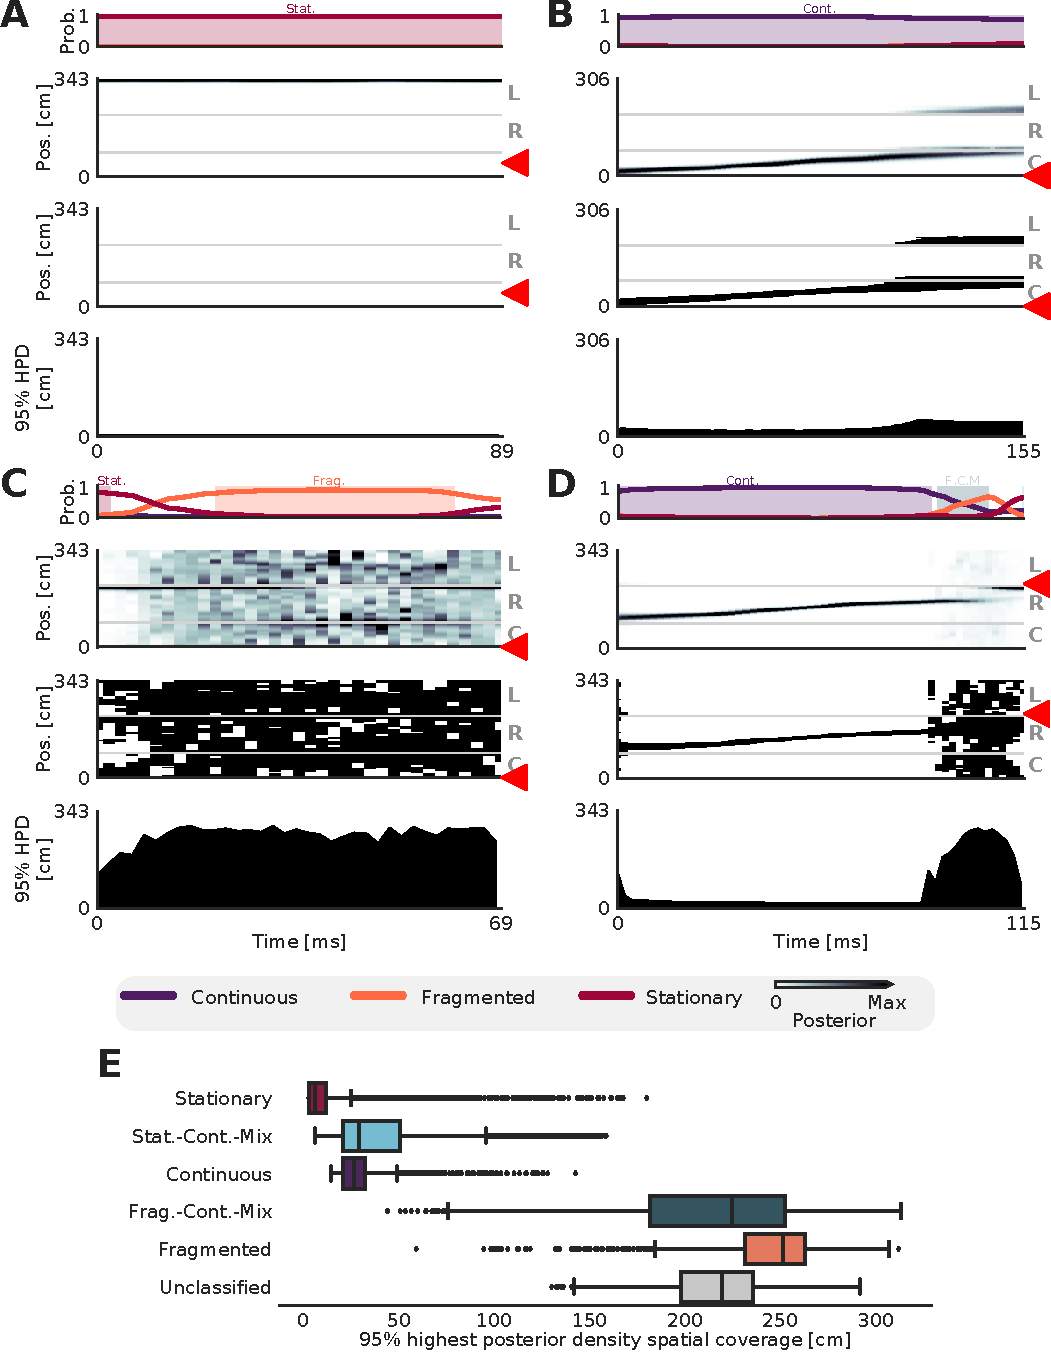
\includegraphics[width=0.80\linewidth]{figures/Figure4/Figure4_v5}
\caption{95 \% Highest Posterior Density of the Dynamics. \textbf{(A-D)}  Examples of the 95 \% Highest Posterior Density. Top panel. Probability of dynamic over time. Shading and labels indicates dynamic categories. 2nd panel. Posterior linear position over time. Red triangle indicates animal's position. 3rd panel. Black indicates the position bin is in the 95\% highest posterior density (HPD) values. 4th panel. Cumulative HPD. \textbf{(E)} Average Cumulative 95\% HPD for each dynamic category.}
\label{4}
\end{figure*}

\subsection*{Many replay trajectories have slower movement speeds}
\begin{figure*}%[tbhp]
\centering
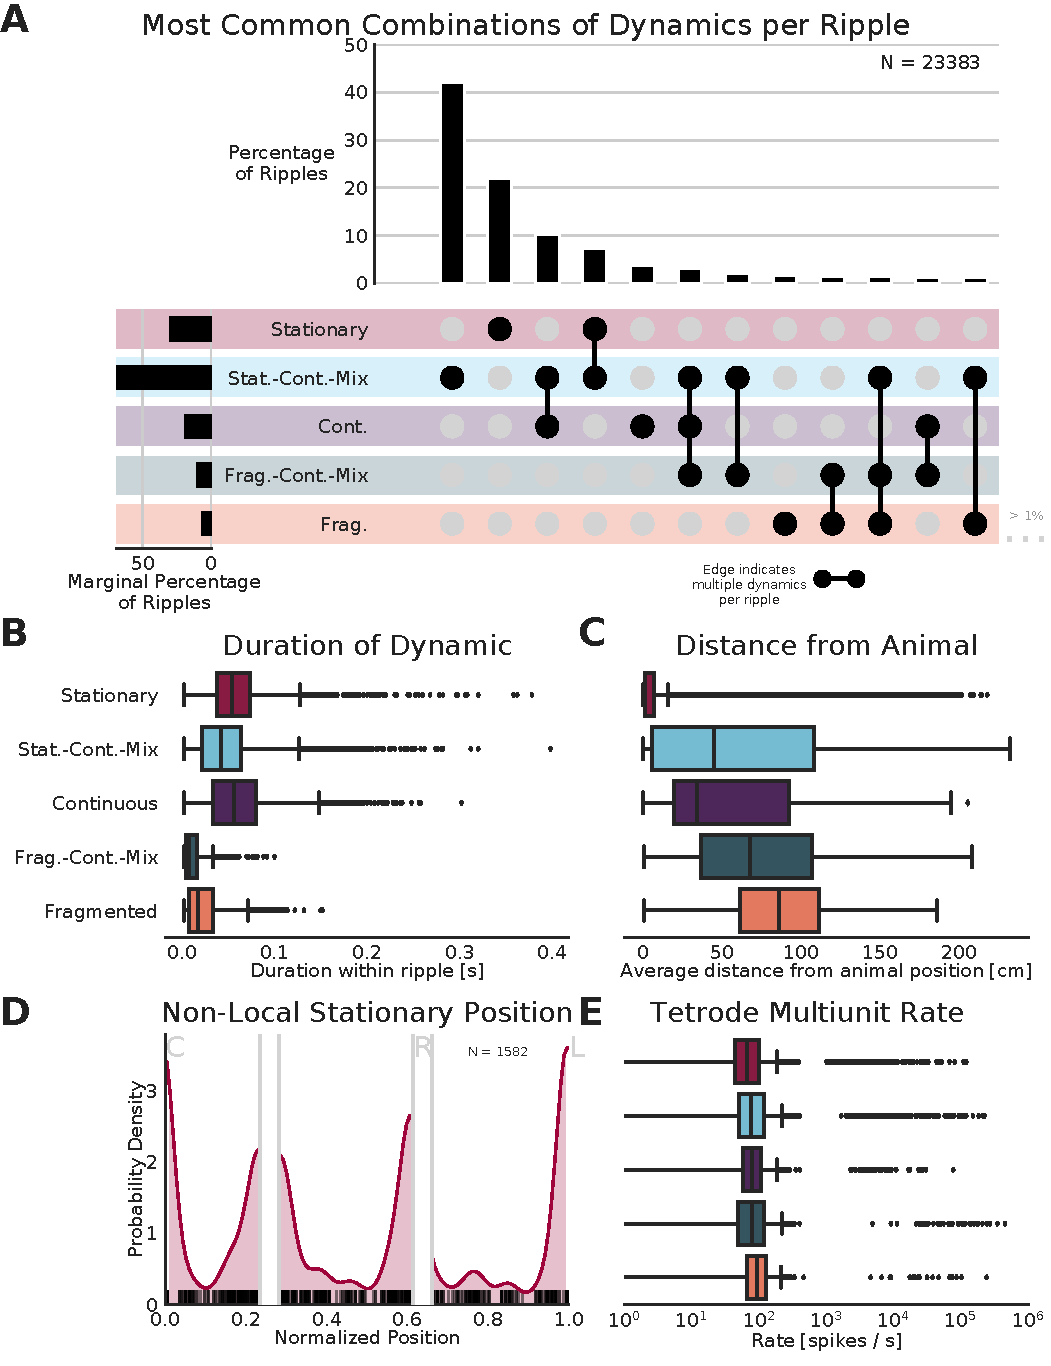
\includegraphics[width=0.80\linewidth]{figures/Figure5/Figure5_v3}
\caption{
Analysis of SWRs from all animals. \textbf{(A)} UpSet plot---which is similar to a Venn diagram with more than 3 sets---of the most common sets of dynamics within each ripple. Each row represents a possible category present in the SWR. Each column represents a set of dynamics categories, where filled-in black dots with an edge between the dots indicates that multiple categories are present in the SWR (at temporally distinct times). The sets are ordered by how often they occurred as indicated by the bar plot above each category. The total number of each category is indicated by the rotated bar plot on the left. \textbf{(B)} Distribution of the duration of each dynamic category within a SWR. \textbf{(C)} The distance of the average latent position from the animal's position for each dynamic category within each SWR. \textbf{(D)} Position of stationary trajectories on the W-track at least 30 cm away from the animal's position. \textbf{(E)} Distribution of multiunit spike rates for each dynamic category within each SWR.
}
\label{5}
\end{figure*}

Our results indicate that most events with coherent spatial content are not continuous; that is, trajectories that move many times the running speed of the animal. We therefore examined these events in more detail. We first noted that most of the SWRs (16454 of 23382 classified SWRs or 70\%) were well described by a single dynamic. Surprisingly, the most common SWRs were categorized exclusively as stationary-continuous mixtures (9860 of 23382 classified SWRs or 42\%, Figure \ref{5}A). These events contain representations that move at rates more consistent with real-world movement (Fig. 1G), but were slightly shorter, on average, than events with continuous dynamics (median duration: stationary-continuous-mixture 72 ms vs. continuous 95 ms, Figure \ref{5}B). Nonetheless, both these slow-moving events and continuous events represented locations that were some distance away from the animal (mean trajectory distance from animal's position: stationary-continuous-mixture 51 cm vs. continuous 42 cm, Figure \ref{5}C). This indicates that the trajectories of these SWRs, like ones that have faster continuous dynamics, do not represent the animal's actual position. 

The next most common category is those SWRs that were exclusively stationary (5149 of 23382 or 22\%). Unlike the stationary-continuous mixtures, most of these events represented a location close to the the animal's actual position (Figure \ref{5}C). There were, however, a number of stationary events  that represented positions far from the animal. We set a threshold of 30 cm distance from the animal to identify "non-local stationary trajectories" and found these trajectories in 1585 of 23382 (~7\%) of classified SWRs. About half of these (731 classified SWRs) were stationary throughout the duration of the SWR. These non-local stationary trajectories most commonly represented reward wells or choice points (Figure \ref{5}D), consistent with \cite{JaiDistincthippocampalcorticalmemory2017}, but a small portion of these trajectories occurred at other locations of the track. This suggests that these representations can be flexibly deployed to represent discrete locations.

Finally, we examined the overall activity levels across dynamics. We found that all the dynamics had similar average tetrode multiunit spiking rates (Figure \ref{5}E). This indicates that all dynamics, including the slower dynamics such as stationary and stationary-continuous mixtures, were driven by sustained spiking information and could not be explained by the absence of spiking.

\section*{Discussion}
Here we developed a state space model that identifies and quantifies generative activity in terms of a mixture of three movement dynamics: stationary, continuous, and fragmented. We showed that this model is interpretable; it has well-defined parameters and allows us to explain a large fraction of SWRs in terms of these dynamics---far greater than had been explained before. We showed that this model is flexible; it can be used with sorted or clusterless spikes, it can be used with 1D or 2D positions, and---because it uses a mixture of dynamics---it allowed us to confidently discover SWRs with non-constant speed and non-linear trajectories that would be difficult to characterize with the typical Bayesian decoder. Finally, we showed that this model is robust; it was relatively insensitive to transition parameters and depended strongly on the hippocampal place representation structure.

Using this model, we found that most SWRs contained spatially coherent content. Importantly, this content was not predominantly trajectories that occurred at many times the speed of the animal, but trajectories that were much closer to the animal's actual movement speed. Many of these events did not simply represent the animal's current location, but other locations on track. 

Our results challenge the notion that hippocampal replays are necessarily many times the speed of the animal. Are stationary events during SWR that represent the animal's position different from stationary events that represent non-local positions

Why our results are different from the Bayesian decoder
seek to describe as many SWR events, clusterless decoding, more permissive model with different dynamics, explicit descriptive model instead of implicit noisy model, smaller time bins

Our results complement those of Stella and colleagues \cite{StellaHippocampalReactivationRandom2019} who found that hippocampal replay trajectories followed Brownian-like diffusion dynamics. We found that  We also clarify how these results can coexist with Pfeiffer and Foster \cite{PfeifferAutoassociativedynamicsgeneration2015} who found that a subset of replay trajectories alternated between stationary and jumpy representations. We also found a log normal distribution of speeds, but it should be noted that they presented their results in terms of  at least for our task, these jumpy representations are relatively rare.



Our model is similar to the competing temporal models approach of Johnson and Redish 2008 \cite{JohnsonMeasuringdistributedproperties2008}, but allows for more . Our model also represents a middle ground between Hidden Markov-style models \cite{MaboudiUncoveringtemporalstructure2018, ChenBayesiannonparametricmethods2016, LindermanBayesiannonparametricapproach2016, ChenUncoveringspatialtopology2012}, which seek to be environment-agnostic discovers of sequential patterns but require a lot of data, and typical Bayesian decoder, which has very restrictive assumptions about the nature of the trajectories. allows SWR to quickly be identified because of the discrete states. Can work in 2D. Can precisely identify timing of dynamics because of acausal decoding

We believe our model can enable a richer set of analyses that takes advantage of all the data, 
The model can easily be extend to incorporate other previously experienced environments by training place field models on those environments and including the appropriate movement transition matrices for those environments.

\begin{acknowledgements}
\end{acknowledgements}

\section*{References}
\bibliography{refs}

\onecolumn
\newpage

\section*{Methods}

\subsection*{Simulated Data}
Encoding data for Figure \ref{1} and Figure \ref{fig:Figure1-Figure supplement 1} was generated by simulating 15 traversals of a 180 cm linear track. The spiking of 19 neurons was simulated using an inhomogeneous Poisson process where the instantaneous firing rate of each neuron changes according to a Gaussian place field. The Gaussian place fields had a variance of 36 cm and were spaced at 10 cm intervals over the 180 cm track. The decoding data for Figure \ref{1}G was generated by simulating 20,000 linear traversals of the 180 cm track, each with a unique constant speed, starting at 0.5 cm/s and increasing by 0.5 cm/s up to 10,000 cm/s. Each simulated neuron "spiked" when the traversal passed through the peak location of its place field.

\subsection*{Recording Locations and Techniques}
Ten male Long Evans rats (500-700 g, 4-9 months old) were trained on a W-track spatial alternation task. 9 rats contributed to previous studies \cite{KarlssonAwakereplayremote2009, KayConstantSubsecondCycling2020, Kayhippocampalnetworkspatial2016, CarrTransientSlowGamma2012}. Neural activity was recorded in CA1, CA2, CA3, MEC, Subiculum, and DG depending on the rat. We only used hippocampal tetrodes (CA1, CA2, CA3) in this study.

\subsection*{Behavioral Task}
All animals performed a W-track spatial alternation task, which is described in detail in \cite{KarlssonAwakereplayremote2009}. In brief, each day, animals alternated between 20 minute rest epochs in a rest box and 15 minutes run epochs in the W-track. On the W-track, animals alternated between two types of runs: inbound and outbound. On inbound runs, the animal had to run from an outer arm to the center arm. On outbound runs, the animals had to run from the center arm to the least recently visited outer arm. Animals were rewarded for performing the task correctly. Only run epochs with at least 9 putative hippocampal pyramidal cells that fired at least 100 spikes were included in the analysis.

\subsection*{Position of the Animal and Linearization}
The animal's 2D position was estimated from digital video (30 Hz) of two infrared diodes placed on the head stage preamplifiers using a semi-automated analysis. In order to decrease the time it takes to run the model, the 2D position of the animal was converted into a 1D position. This is done by first defining a 2D graph representation of the track (herein referred to as the track graph), where edges correspond to segments of the W-track and nodes represent intersection points between those segments. Then, based on the algorithm in \cite{NewsonHiddenMarkovmap2009}, we use a Hidden Markov Model (HMM) to classify the most likely track segment the animal is on. Using the HMM takes into account the time dependent nature of the data and helps prevents sudden jumps from one track segment to another, which is particularly important near intersections. The observation model of the HMM is Gaussian and it models the likelihood of being on a track segment as the Gaussian distance to that segment with a 5 cm standard deviation. The state transition model is an empirically estimated state transition that changes with each time point that tries to ensure that the Euclidean distance between successive position estimates is similar to the shortest path distance along the graph between successive position estimates. A slight bias of 0.1 is given to the diagonal to encourage staying on the same track segment. The most likely track segment the animal is on is computed using the Viterbi algorithm. After finding the track segment that corresponds to each 2D position, the 2D position is projected onto the track segment. This allows us to define a distance from the center well in terms of shortest path length on the track, where 0 cm represents the center well position. The linear distance can then be converted into a linear position by assigning each track segment a position in 1D space. 15 cm gaps were placed between the center arm, left arm, and right arms in 1D space to prevent any smoothing done in the model from bleeding over inappropriately. The code used for linearization can be found at \url{https://github.com/Eden-Kramer-Lab/loren_frank_data_processing}.

\subsection*{Sorted Spikes, Multiunit Spikes and Waveform Features}
To obtain the neural data used for decoding, hippocampus electrical potentials were recorded at 30 kHz, referenced to a corpus callosum tetrode, and then digitally filtered between 600 Hz and 6 kHz. Events were considered threshold crossing events if any one of the four tetrode wires exceeded a 60 $\mu V$ threshold. These multiunit threshold crossing events and the associated peak amplitudes of the tetrodes wires---defined as the electrical potential value at the time of the maximum amplitude at the threshold crossing---were used as data for the clusterless version of the model.

For decoding using sorted spikes, the multiunit events were processed further to assign events to putative single cells. Putative single cells were manually identified based on the clustering of three waveform features within a day: peak amplitude, principal components, and spike width. Only putative hippocampal pyramidal cells---identified based on spike width and average firing rate---were included in the analysis.

\subsection*{SWR Detection}
Sharp wave ripples were detected using the same method as in \cite{Kayhippocampalnetworkspatial2016}. Each CA1 LFP was obtained by downsampling the original 30 kHz electrical potential to 1.5 kHz, bandpass filtering between 0.5 Hz and 400 Hz. This was further bandpass filtered between 150-250 Hz for ripple band frequencies, squared and then summed across tetrodes---forming a single population trace over time. This trace was smoothed with a Gaussian with a 4 ms standard deviation and the square root of this trace was taken to get an estimate of the population ripple band power. Candidate SWR times were found by z-scoring the population power trace and finding times when the z-score exceeded 2 standard deviations for a minimum of 15 ms and the speed of the animal was less than 4 cm/s. The SWR times were then defined as times when the z-score was greater than the mean and contained the candidate SWR times. The code used for ripple detection can be found at \url{https://github.com/Eden-Kramer-Lab/ripple_detection}.

\subsection*{The Model}
Let $x_{k}$ be a continuous latent variable that corresponds to the position represented by the population of cells at time $t_k$ and $I_{k}$ be a discrete latent variable that is an indicator for the dynamics we wish to characterize: stationary, continuous, and fragmented. The goal of the model is to simultaneously estimate the posterior probability of position and dynamics $p(x_k, I_k \mid O_{1:T})$, where $O_{1:T}$ corresponds to the observed spiking data from time 1 to time $T$. The observed data can be either spike trains $\Delta N_{1:T}^{(1:C)}$ from $C$ putative cells when decoding with sorted spikes or multiunit spikes $\Delta N_{1:T}^{(1:E)}$ and their associated wave form features $\Vec{m}$ from each tetrode $E$ when decoding with clusterless spikes.

We have previously shown \cite{DenovellisCharacterizinghippocampalreplay2019} that the posterior probability $p(x_k, I_k \mid O_{1:T})$ can be estimated by applying the following recursive causal filter equation, starting with initial conditions $p(x_{0}, I_{0} \mid O_{0})$ and iterating to time T:

$$
p(x_{k}, I_{k} \mid O_{1:k}) \propto
p(O_{k}  \mid x_{k}, I_{k}) \sum_{I_{k-1}} \int p(x_{k} \mid x_{k-1}, I_{k}, I_{k-1}) 
Pr(I_{k} \mid I_{k-1}) p(x_{k-1}, I_{k-1} \mid O_{1:k-1}) dx_{k-1}
$$
and then applying the acausal smoother equation, starting from the last estimate of the casual filter $p(x_{T}, I_{T} \mid O_{1:k})$ and recursively iterating backwards to time 1:
$$
p(x_{k}, I_{k} \mid O_{1:T}) =
p(x_{k}, I_{k} \mid O_{1:k})
\sum_{I_{k+1}} \int \frac{p(x_{k+1} \mid x_{k}, I_{k+1}, I_{k})
Pr(I_{k+1} \mid I_{k})}{p(x_{k+1}, I_{k+1} \mid O_{1:k})}
p(x_{k+1}, I_{k+1} \mid O_{1:T}) dx_{k+1}
$$
where:
$$
p(x_{k+1}, I_{k+1} \mid O_{1:k}) =
\sum_{I_{k}} \int p(x_{k+1} \mid x_{k}, I_{k+1}, I_{k}) Pr(I_{k+1} \mid I_{k})
p(x_{k}, I_{k} \mid O_{1:k}) dx_{k}
$$

Therefore, to specify the model, we have to define or estimate the following quantities:
\begin{enumerate}
  \item $p(x_{0}, I_{0})$ - the initial conditions
  \item $Pr(I_{k} \mid I_{k-1})$ - the dynamics transition matrix
  \item $p(x_{k} \mid x_{k-1}, I_{k}, I_{k-1})$ - the dynamics movement model
  \item $p(O_{k}  \mid x_{k}, I_{k})$ - the likelihood of the observations
\end{enumerate}

For the initial conditions $p(x_{0}, I_{0})$, we set each dynamic $I_0$ to have uniform probability over all possible positions $\mathcal{U}(\min x, \max x)$, reflecting the fact that we do not have any prior knowledge about which dynamic or position is more likely:

\begin{equation*}
  p(x_{0}, I_{0}) = 
  \begin{blockarray}{*{1}{c} l}
    \begin{block}{[*{1}{c}]>{$\footnotesize}l<{$}}
      \mathcal{U}(\min x, \max x) \bigstrut[t]& $I_{0} = Stationary$ \\
      \mathcal{U}(\min x, \max x) & $I_{0} = Continuous$ \\
      \mathcal{U}(\min x, \max x) & $I_{0} = Fragmented$ \\
    \end{block}
  \end{blockarray}
\end{equation*}

For the dynamics transition matrix $Pr(I_{k} \mid I_{k-1})$, which defines how likely the dynamic is to change to another dynamic versus persist in the same dynamic, we set it to be:

\begin{equation*}
  Pr(I_{k} \mid I_{k-1}) = 
  \begin{blockarray}{*{3}{c} l}
    \begin{block}{*{3}{>{$\footnotesize}c<{$}} l}
      $I_{k} = Stationary$ & $I_{k} = Continuous$ & $I_{k} = Fragmented$ \\
    \end{block}
    \begin{block}{[*{3}{c}]>{$\footnotesize}l<{$}}
      0.98 & 0.01 & 0.01 \bigstrut[t]& $I_{k-1} = Stationary$ \\
      0.01 & 0.98 & 0.01 & $I_{k-1} = Continuous$ \\
      0.01 & 0.01 & 0.98 & $I_{k-1} = Fragmented$ \\
    \end{block}
  \end{blockarray}
\end{equation*}

to encode the prior expectation that each of the dynamics will last the average duration of 100 ms, with a small probability of changing to one of the other dynamics.

For the dynamics movement model $p(x_{k} \mid x_{k-1}, I_{k}, I_{k-1})$, which defines how likely the position $x_{k}$ is to change given the previous position $x_{k-1}$ and current $I_{k}$ and past dynamics $I_{k-1}$, we set it to be:

\begin{equation*}
  p(x_{k} \mid x_{k-1}, I_{k}, I_{k-1}) = 
  \begin{blockarray}{*{3}{c} l}
    \begin{block}{*{3}{>{$\footnotesize}c<{$}} l}
      $I_{k} = Stationary$ & $I_{k} = Continuous$ & $I_{k} = Fragmented$ \\
    \end{block}
    \begin{block}{[*{3}{c}]>{$\footnotesize}l<{$}}
      \delta(x_{k-1}) & \mathcal{N}(x_{k-1}, 6.0) & \mathcal{U}(\min x, \max x) \bigstrut[t]& $I_{k-1} = Stationary$ \\
      \delta(x_{k-1}) & \mathcal{N}(x_{k-1}, 6.0)  & \mathcal{U}(\min x, \max x) & $I_{k-1} = Continuous$ \\
      \mathcal{U}(\min x, \max x) & \mathcal{U}(\min x, \max x) & \mathcal{U}(\min x, \max x) & $I_{k-1} = Fragmented$ \\
    \end{block}
  \end{blockarray}
\end{equation*}
where $\delta(x_{k-1})$ is an identity transition matrix where position cannot change from the previous time step, $\mathcal{N}(x_{k-1}, 6.0)$ is a random walk from the previous position with variance 6.0, and $\mathcal{U}(\min x, \max x)$ is a uniform transition that allows transitions to any possible position. As discussed in the Results, this says that when persisting in the same dynamic, the stationary, continuous, and fragmented dynamics are defined by the identity transition, the random walk, and the uniform transition, respectively. When transitioning to or from the fragmented dynamic, we assume we do not have any information about the position, so the transition is uniform. Finally, when the transition is from the stationary to continuous, we assume the position is spatially close where it was previously, so we use a random walk. When the transition is from continuous to stationary, we assume that the position is no longer changing, so we use the identity transition.

Lastly, we evaluate the likelihood of the observations $p(O_{k} \mid x_{k}, I_{k})$ based on an encoding model fit during the encoding period. We assume the likelihood is the same for each dynamic $I_k$, so we only need to evaluate $p(O_{k} \mid x_{k})$. It has been shown \cite{ZhangInterpretingNeuronalPopulation1998, BrownStatisticalParadigmNeural1998} that the Poisson likelihood with sorted spikes can be computed as:
$$
p(O_{k} \mid x_{k}) = p(\Delta N_{k}^{(1:C)} \mid x_{k}) \propto
\prod^{C}_{i=1} [\lambda_{i}(t_{k} \mid x_{k})\Delta_{k}]^{N_{t_{k}}^{i}} \\
    \exp[-\lambda_{i}(t_{k} \mid x_{k})\Delta_{k}]
$$
where $N_{t_{k}}^{i}$ represents a spike at time $t_k$ from cell $i$, $\Delta_k$ is the time bin size, and $\lambda_{i}(t_{k} \mid x_{k})$ is the instantaneous firing rate of cell $i$ given position $x_{k}$. $\lambda_{i}(t_{k} \mid x_{k})$ is the "place field" of the cell, which can be estimated by fitting a generalized linear model to each cell's spiking during the encoding period.

Likewise, it has been shown \cite{ChenTransductiveneuraldecoding2012, DengRapidclassificationhippocampal2016, KloostermanBayesiandecodingusing2014} that the clusterless likelihood can be computed as: 
$$
p(O_{k} \mid x_{k}) = p(\Delta N_{k}^{(1:E)}, \vec{m_k} \mid x_{k}) \propto
\prod^{E}_{i=1} [\lambda_{i}(t_{k}, \vec{m}_k \mid x_{k})\Delta_{k}]^{N_{t_{k}}^{i}} \\
    \exp[-\Lambda_{i}(t_{k} \mid x_{k})\Delta_{k}]
$$
where $\lambda_{i}(t_{k}, \vec{m}_k \mid x_{k})$ is now a generalized firing rate that depends on an associated wave form features $\Vec{m}$ and $\Lambda_{i}(t_{k} \mid x_{k})$ is a marginal firing rate that is equivalent to a place field estimated on multiunit spikes. Both of these rates can be defined as:
$$
\lambda_{i}(t_{k}, \vec{m}_k \mid x_{k}) = \mu_i \frac{p_{i}(x_k, \vec{m}_k)}{\pi(x)}
$$
and
$$
\Lambda_{i}(t_{k} \mid x_{k}) = \mu_i \frac{p_{i}(x_k)}{\pi(x)}
$$
where $\mu_i$ is the mean firing rate for tetrode $i$, $\pi(x)$ is the spatial occupancy of the animal on the track, and $p_{i}(x_k, \vec{m}_k)$ and $p_{i}(x_k)$ are the joint probability of observing waveform features $\Vec{m}$ and position $x$ and the probability of observing position $x$, respectively. $\pi(x)$, $p_{i}(x_k, \vec{m}_k)$, $p_{i}(x_k)$ can all be estimated by training a kernel density estimator on each tetrode's spike waveform features and corresponding position during the encoding period.

\subsection*{Encoding - Sorted Spikes}
In order to encode how each cell's spiking activity relates to position (the place field), we fit a generalized linear model (GLM) with a Poisson response distribution to each cell's spiking activity during the encoding period, which we define as all movement times (time periods when the running speed is greater than 4 cm/s). We estimate the parameters $\beta$, which consist of $\beta_{0}$, the average firing rate over time, and $\beta_{i}$, weights for third degree B-splines basis functions $f_{i}$ over position (or tensor products of the B-splines when position is two dimensional). B-spline basis functions are used because place field firing activity is assumed to vary smoothly over position and this prior knowledge can be exploited to reduce the total number of model parameters needed. Each basis function is spaced every 5 cm over the range of the position and zero constrained so that the change encoded by the parameters is relative to the baseline firing rate. We use a log link function to convert the linear combination of parameters to an instantaneous firing rate over time $\lambda(t)$ to ensure the rate is always positive. 

$$log(\lambda(t)) = \beta_{0} + \sum_{i} f_{i}(position)\beta_{i}$$

A small L2 penalization term $-\lambda\|\beta_{i}\|_{2}^{2}$ used to prevent model fitting instability when spiking activity is very low. We set this to 0.5 for all cells. Fitting is done by maximizing the penalized likelihood using a Newton-Raphson algorithm. The code used to fit the GLMs is available at \url{https://github.com/Eden-Kramer-Lab/regularized_glm}.

\subsection*{Encoding - Clusterless}
In order to encode how each tetrode's unsorted spiking activity and waveform features relate to position, we used kernel density estimation (KDE) to estimate the following distributions: $\pi(x)$, $p_{i}(x_k)$, and $p_{i}(x_k, \vec{m}_k)$. We used KDEs of the form: 
$$
kde(y) = \frac{1}{N h_1...h_D} \sum^{N}_{i=1} \prod^{D}_{d=1} K_{d}\left(\frac{y_d - y_{i,d}}{h_d}\right)
$$
where $y$ is the data with $D$ dimensions, $K$ is a 1 dimensional Gaussian kernel with bandwidth $h_d$, $y_{i, d}$ is the data observed during movement, $N$ is the number of observations during the movement period. For $\pi(x)$, $y_{i, d}$ is all positions observed during movement. For $p_{i}(x_k)$, $y_{i, d}$ is all positions at the time of multiunit spikes during movement. For $p_{i}(x_k, \vec{m}_k)$, $y_{i, d}$ is all positions at the time of multiunit spikes and their associated waveform features during movement. We choose the bandwidth $h_d$ to be 6.0 cm for any position dimension and 24.0 $\mu V$ for any spike amplitude dimension, because these parameters minimized decoding error in \cite{KloostermanBayesiandecodingusing2014}. The mean firing rate $\mu_k$ was also estimated during movement.

\subsection*{Decoding}
In order to decode $p(x_{k}, I_{k} \mid O_{1:T})$, we used a grid based approximation of the latent position $x_k$ that respected the geometry of the track. For 1D linearized positions, we discretized the position space based on the same track graph we used for linearization by finding bins less than or equal to the chosen position bin size for each edge of the graph. For 2D positions, we discretized the position space by binning 2D positions occupied by the animal with equal sized bins of the chosen position bin size, followed by morphological opening to get rid of any holes smaller than the bin size. This was done using Scipy image processing tools \cite{SciPy1.0ContributorsSciPyfundamentalalgorithms2020}. This grid based approximation allows us to use Reimann sums to approximate the integrals in the causal filter and acausal smoother equations. We chose a position grid with bins of 3 cm in width (and height if the model was computed with 2D positions) in order to get good resolution for the random walk transition matrices (which had 6 cm variance) as well as for the clusterless and sorted spikes decoding (which have 6 cm bandwidth for the KDE position dimensions and 5 cm spline knots for the GLM). For sorted spikes decoding, we evaluated the place field $\lambda_{i}(t_{k} \mid x_{k})$ on the midpoint of these bins. Likewise, for clusterless decoding, we evaluated the spike amplitudes observed during the decoding period by evaluating the KDE for $p_{i}(x_k, \vec{m}_k)$ for the midpoint of these bins.

We also used this grid bins in combination with the track graph in order to construct the appropriate 1D random walk transition matrices that respected the track geometry. To do this, we inserted the bin centers as nodes in the track graph, and then computed the shortest path distance between all pairs of position bin centers. We then evaluated a zero mean Gaussian with a variance of 6 cm on these distances to get the appropriate transition probability of moving from bin to bin.

Finally, for our SWR analysis of $p(x_{k}, I_{k} \mid O_{1:T})$, we decoded each immobility time periods (times when the animal's speed was < 4 cm / s) in 2 ms time bins and extracted the SWR times.

\subsection*{Mixture probability of the dynamics}
The mixture probability of the dynamics is a quantity that indicates how much that dynamic is contributing to the posterior at a given time. We estimate the mixture probability of the dynamics by integrating out position the joint posterior:
$$Pr(I_{k} \mid O_{1:T}) = \int p(x_{k}, I_{k} \mid O_{1:T}) dx_{k}$$
As in other calculations, the integral is approximated with a Reimann sum.

\subsection*{Posterior probability of position}
The posterior probability of position is a quantity that indicates the most probable "mental" positions of the animal based on the data. We estimate it by marginalizing the joint probability over the dynamics.
$$p(x_{k} \mid O_{1:T}) = \sum_{I_{k}} p(x_{k}, I_{k} \mid O_{1:T})$$

\subsection*{Classification of Dynamics}
We used a threshold of 0.8 to classify the probability of each state $Pr(I_{k} \mid O_{1:T})$ into 5 categories. Time periods during sharp wave ripples are labeled as Stationary, Continuous, or Fragmented when the probability of each state is above 0.8. Time periods are labeled as Stationary-Continuous-Mix or Fragmented-Continuous-Mix when the sum of Stationary and Continuous or Fragmented and Continuous are above 0.8, respectively. Time periods where none of these criterion are met are considered unclassified.

\subsection*{Shuffle Analysis of the Effect of Place Encoding on Classification of Dynamics}
In order to confirm that the model classification of dynamics depended on hippocampal place specific encoding, we resampled the position during movement with replacement, but preserved the spike times and spike waveform amplitudes. We fit the clusterless encoding model on the resampled data and then decoded the immobility periods. Like with the non-resampled data, we then extracted the SWR times and determined their classification based on our classification scheme. We repeated this shuffle analysis 50 times and compared this distribution to the real data for two epochs on two different animals (animal Bond, day 3, epoch 2 and animal Remy, day 35, epoch 2).

\subsection*{Highest Posterior Density}
The 95\% highest posterior density (HPD) is a measurement of the spread of the posterior probability and is defined as the region of the posterior that contains the top 95\% values of the posterior probability. In this manuscript, we use the HPD to evaluate the uncertainty of the posterior probability of position. We calculate the 95\% HPD by determining the maximum threshold value $h$ that fulfills the follow equality:
$$
\int_{\{x: p(x_{k} \mid O_{1:T}) > h\}} p(x_{k} \mid O_{1:T})dx = 0.95
$$
The 95\% HPD is the set of position bins with posterior values greater than the threshold $\{x : p(x_{k} \mid O_{1:T}) > h\}$. The cumulative spatial extent of the HPD is calculated by taking the integral of the members of this set:
$$
\int_{\{x: p(x_{k} \mid O_{1:T}) > h\}} \mathbb{1}dx
$$
which we approximate with a Reimann sum.

\subsection*{Replay distance from animal}
Replay distance from the animal is defined as the shortest path distance along the track graph between the animal's 2D position projected on to the track graph (see Linearization) and the MAP estimate of the posterior probability of position $\argmax_{x_k} p(x_{k} \mid O_{1:T})$, which is defined as the center of the position bin with the greatest posterior value. The shortest path is found using Dijkstra's algorithm.

\subsection*{Non-Local Stationary Position}
The non-local stationary position is defined as replay distances at least 30 cm from the animal's position during a time period classified as stationary.

\subsection*{Software and Code Availability}
Python code used for analysis and generating figures in the paper is available at: \url{https://github.com/Eden-Kramer-Lab/replay_trajectory_paper}. Code for the classifier is available in a separate software repository to facilitate code reuse at: \url{https://github.com/Eden-Kramer-Lab/replay_trajectory_classification}. All code is open-source and licensed under the MIT Software License. Classifier code can be easily installed as a python package with all requisite dependencies using pip or conda. See software repositories for specific details.

\newpage

%%%%%%%%%%%%%%%%%%%%%%%%%%%%%
% Supplementary Information %
%%%%%%%%%%%%%%%%%%%%x%%%%%%%%%
\beginsupplement
\captionsetup*{format=largeformat}

\begin{figure*}%[tbhp]
\centering
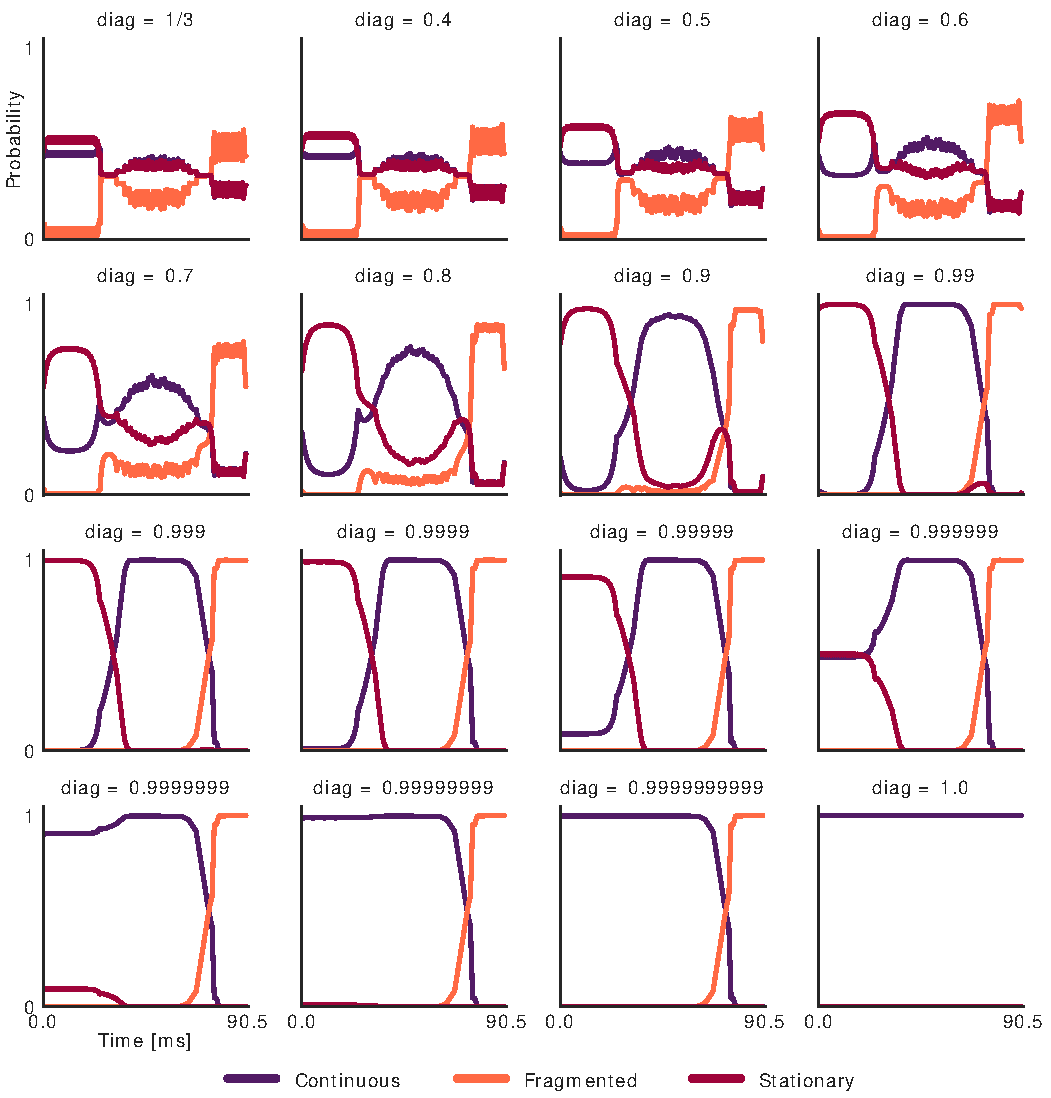
\includegraphics[width=0.80\linewidth]{figures/Figure1-supplemental1/Figure1_v2_supplemental1}
\caption{The model is robust to changes in the discrete transition matrix. Each plot shows the probability of each dynamic on simulated data example from Figure 1 with a different diagonal value--which governs the probability of remaining in that state. The off-diagonal values--the probability of switching to one of the other dynamics--are set to be equally likely with the remainder of the probability, as in Figure 1D. The first plot (upper left) shows the case when all dynamics are equally likely. The diagonal increases from left to right, top to bottom, until the case where the diagonal is one and the off-diagonal is zero--i.e. the case where there is no probability of switching to another state.}
\label{fig:Figure1-Figure supplement 1}
\end{figure*}

\begin{figure*}%[tbhp]
\centering
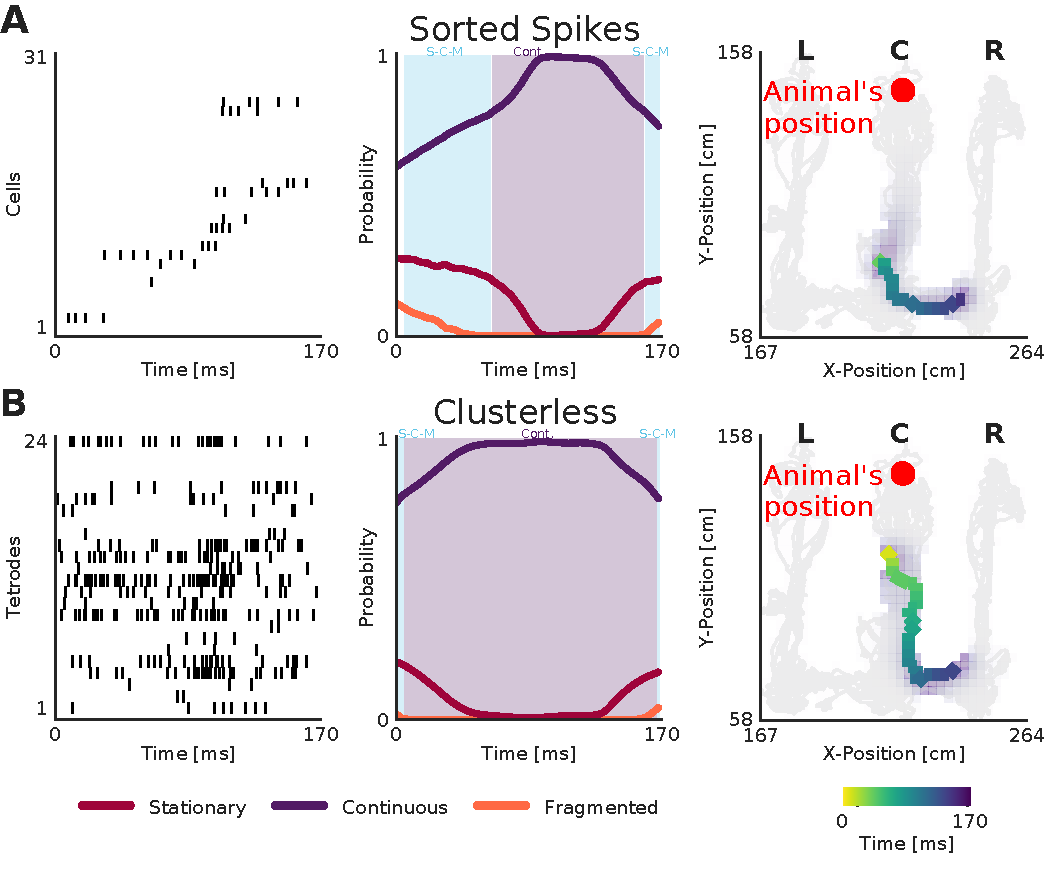
\includegraphics[width=0.80\linewidth]{figures/Figure2-supplemental1/Figure2_v3-supplemental1}
\caption{Decoding the same SWR in Figure 2 using 2D clusterless and sorted spikes. \textbf{(A)} The left plot shows the spikes from cells arranged by the linear position of the peak of place field as in Figure 2. The middle plot shows the probability of each dynamic over time from the 2D decode. Shaded regions indicate classification category as in Figure 1G and 2. The rightmost plot shows the MAP estimate of the latent position with color indicating time. The latent position posterior summed over time is shown in purple underneath. The light grey lines represent the position of the animal over the entire epoch and the red dot represents the animal's position. \textbf{(B)} Same as in A, but with clusterless decoding.}
\label{fig:Figure2-Figure supplement 1}
\end{figure*}

\begin{figure*}%[tbhp]
\centering
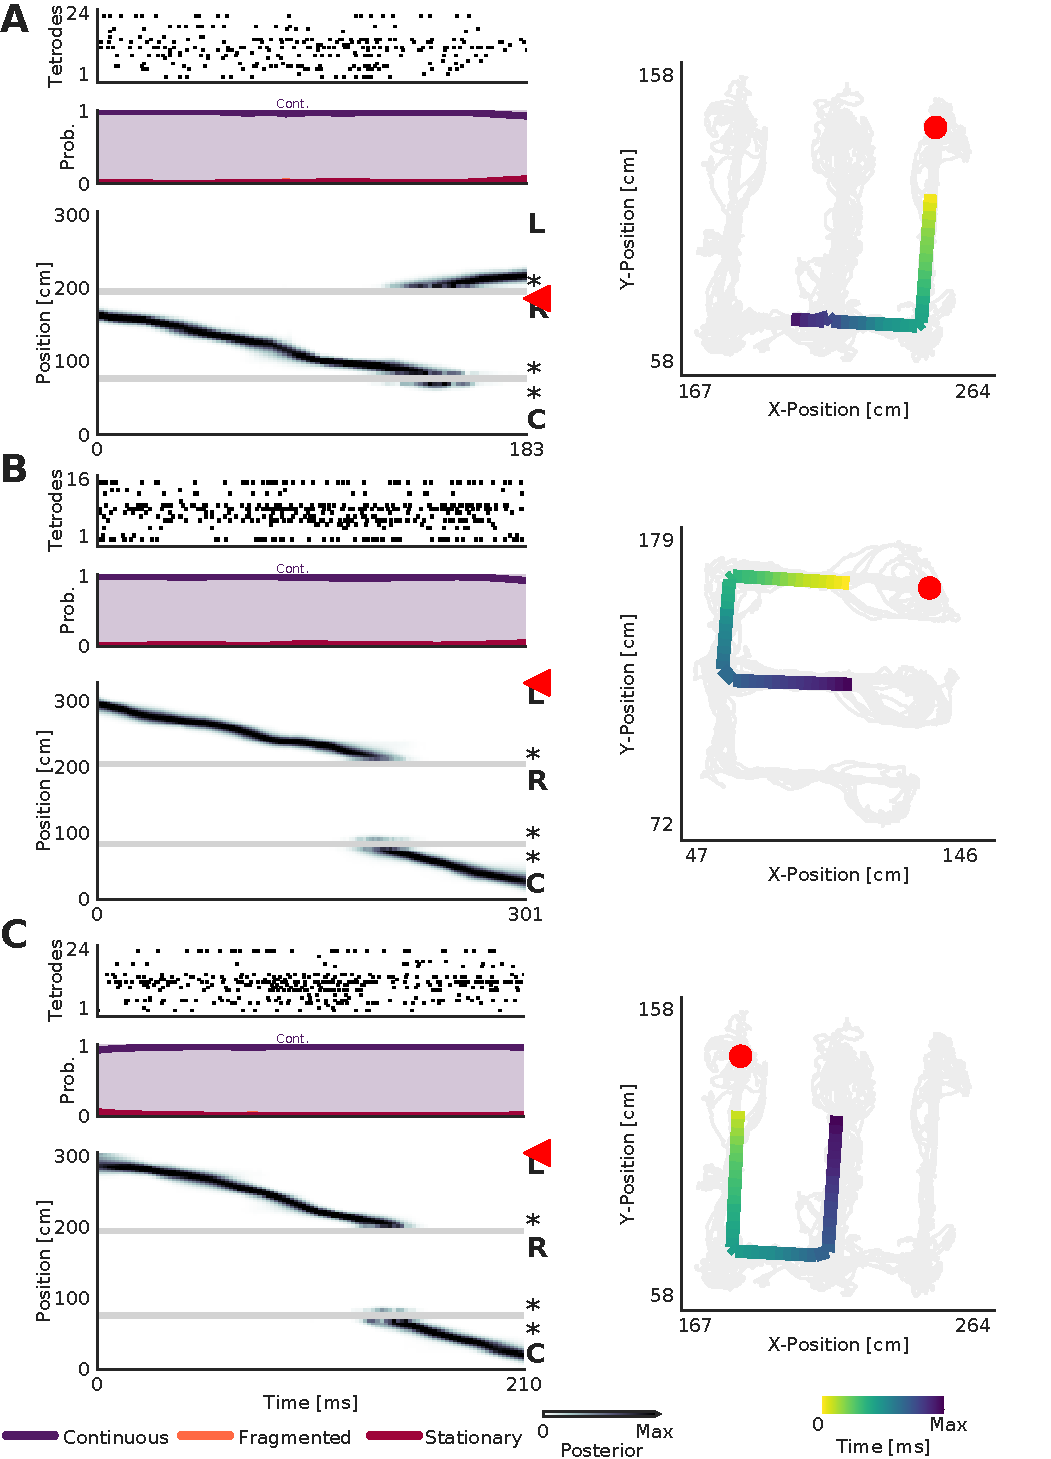
\includegraphics[width=0.80\linewidth]{figures/Figure2-supplemental2/Figure2_v3-supplemental2}
\caption{A-C. Examples of continuous replays. Left panel uses the same conventions as Figure 2A and 2B. Right panel shows the 1D MAP estimate projected back to 2D as in Figure 2C. Color indicates time. Light grey lines indicate the animal's position over the entire epoch.}
\label{fig:Figure2-Figure supplement 2}
\end{figure*}

\begin{figure*}%[tbhp]
\centering
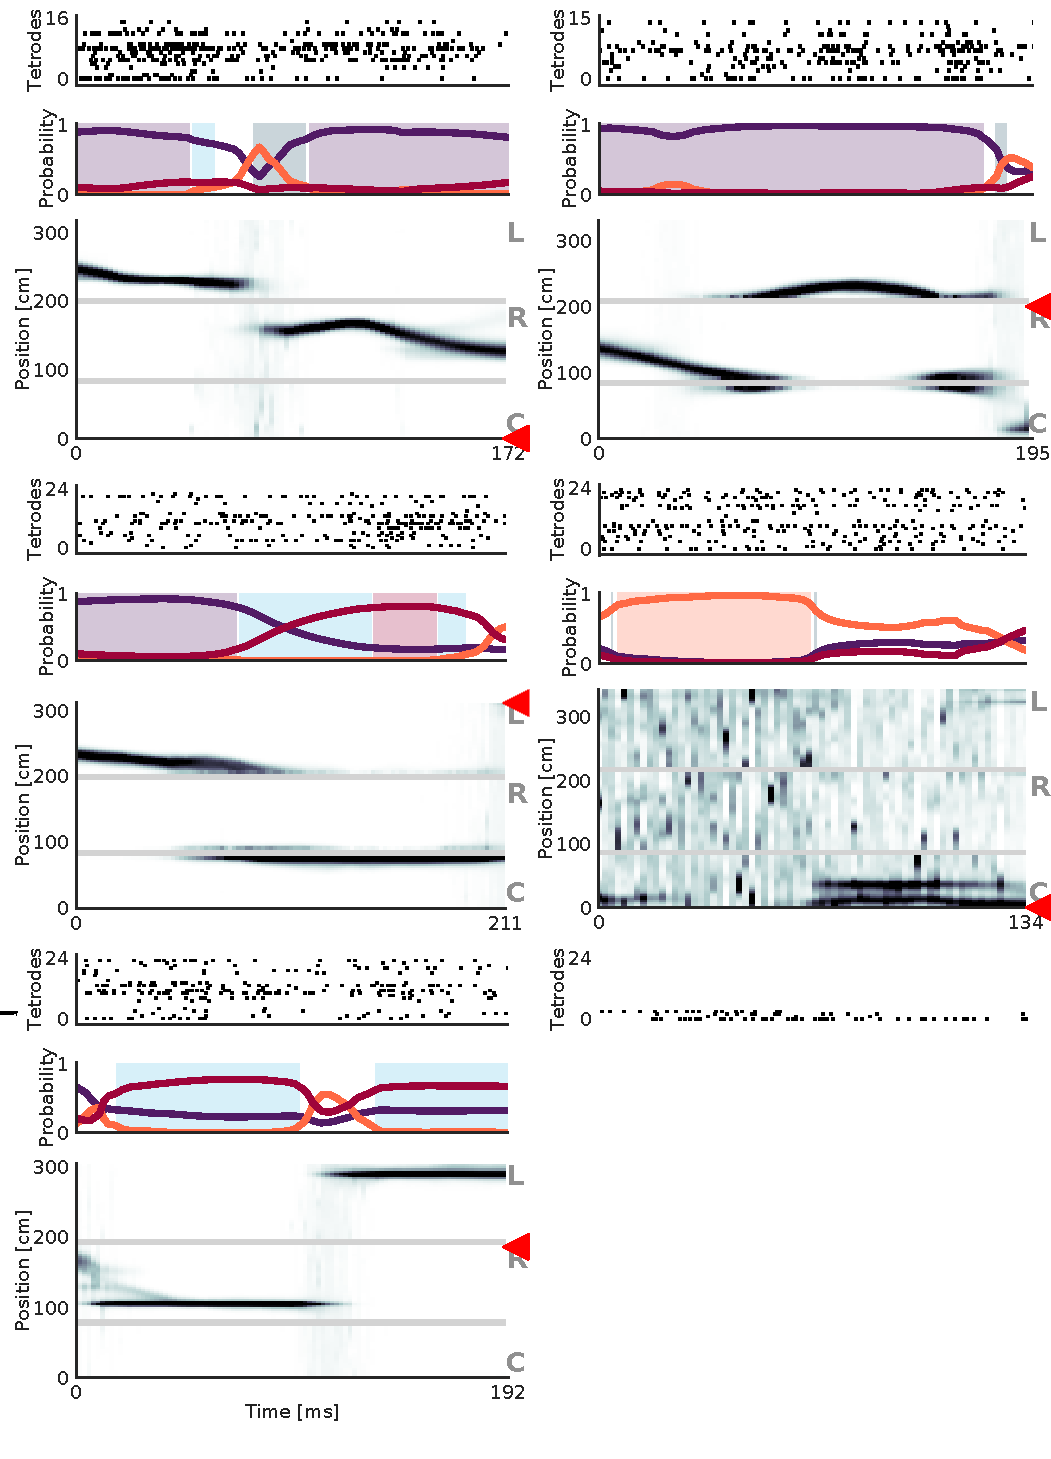
\includegraphics[width=0.80\linewidth]{figures/Figure3-supplemental1/Figure3_v3_supplemental1}
\caption{More examples of replays that would not be well-characterized by using the Bayesian decoder. Conventions are the same as in Figure 3. \textbf{(A)} A continuous replay that starts in the left arm back toward the center well, jumps to the right arm and continuous back toward the center well. \textbf{(B)} A continuous replay that travels down the right arm toward the center well, proceeds past the choice point toward the left well and then returns back to the choice point. \textbf{(C)} A replay that starts down the left arm toward the center arm and turns into a stationary trajectory near the choice point. \textbf{(D)} The first half is a fragmented replay and the second half is unclassified. \textbf{(E)} A stationary trajectory in the first half of the SWR on the right arm and then a stationary trajectory in the SWR at the left well. \textbf{(F)} A stationary trajectory that starts at the animal's position at the center well, then jumps to the left well and comes back toward the center well.
}
\label{fig:Figure3-Figure supplement 1}
\end{figure*}

\begin{figure}%[tbhp]
\centering
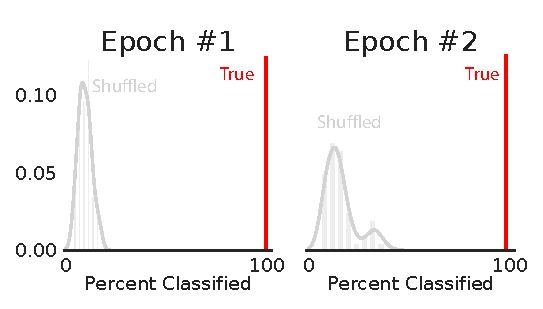
\includegraphics[width=0.80\linewidth]{figures/Figure3-supplemental2/Figure3_v1-supplemental2}
\caption{Comparison of real vs. position shuffled data for two epochs from different animals. Line represents the percent of SWR classified in that epoch for real data. The histogram represents the distribution after 50 shuffles of the position data. Position data was shuffled by resampling with replacement from the set of all observed positions in that epoch, destroying position information but preserving spiking timing.}
\label{Figure3-Figure supplement 2}
\end{figure}

%TC:endignore
%the command above ignores this section for word count

\end{document}

